\chapter{Architektur\label{chap3:Drittes-Kapitel}}

Für die Architektur der mobilen Anwendung \glqq Geogram\grqq{}, wurden die zwei Frameworks \glqq Ionic\grqq{} und \glqq Express\grqq{} und die Entwicklungs-Plattform \glqq Firebase\grqq{} verwendet.

Wie in \autoref{fig:technologie} veranschaulicht, wird das Web-Framework \glqq Ionic\grqq{} für das Frontend verwendet. Das Backend kann in zwei Bereiche unterteilt werden. Zum einen wird die Entwicklungs-Plattform \glqq Firebase\grqq{} und das Node.js Web-Framework \glqq Express\grqq{} verwendet. Genauere Informationen bezüglich der Aufteilung des Backends wird in \autoref{sec3.2:Unterpunkt-2} beschrieben.

\begin{figure}[H]
    \centering
    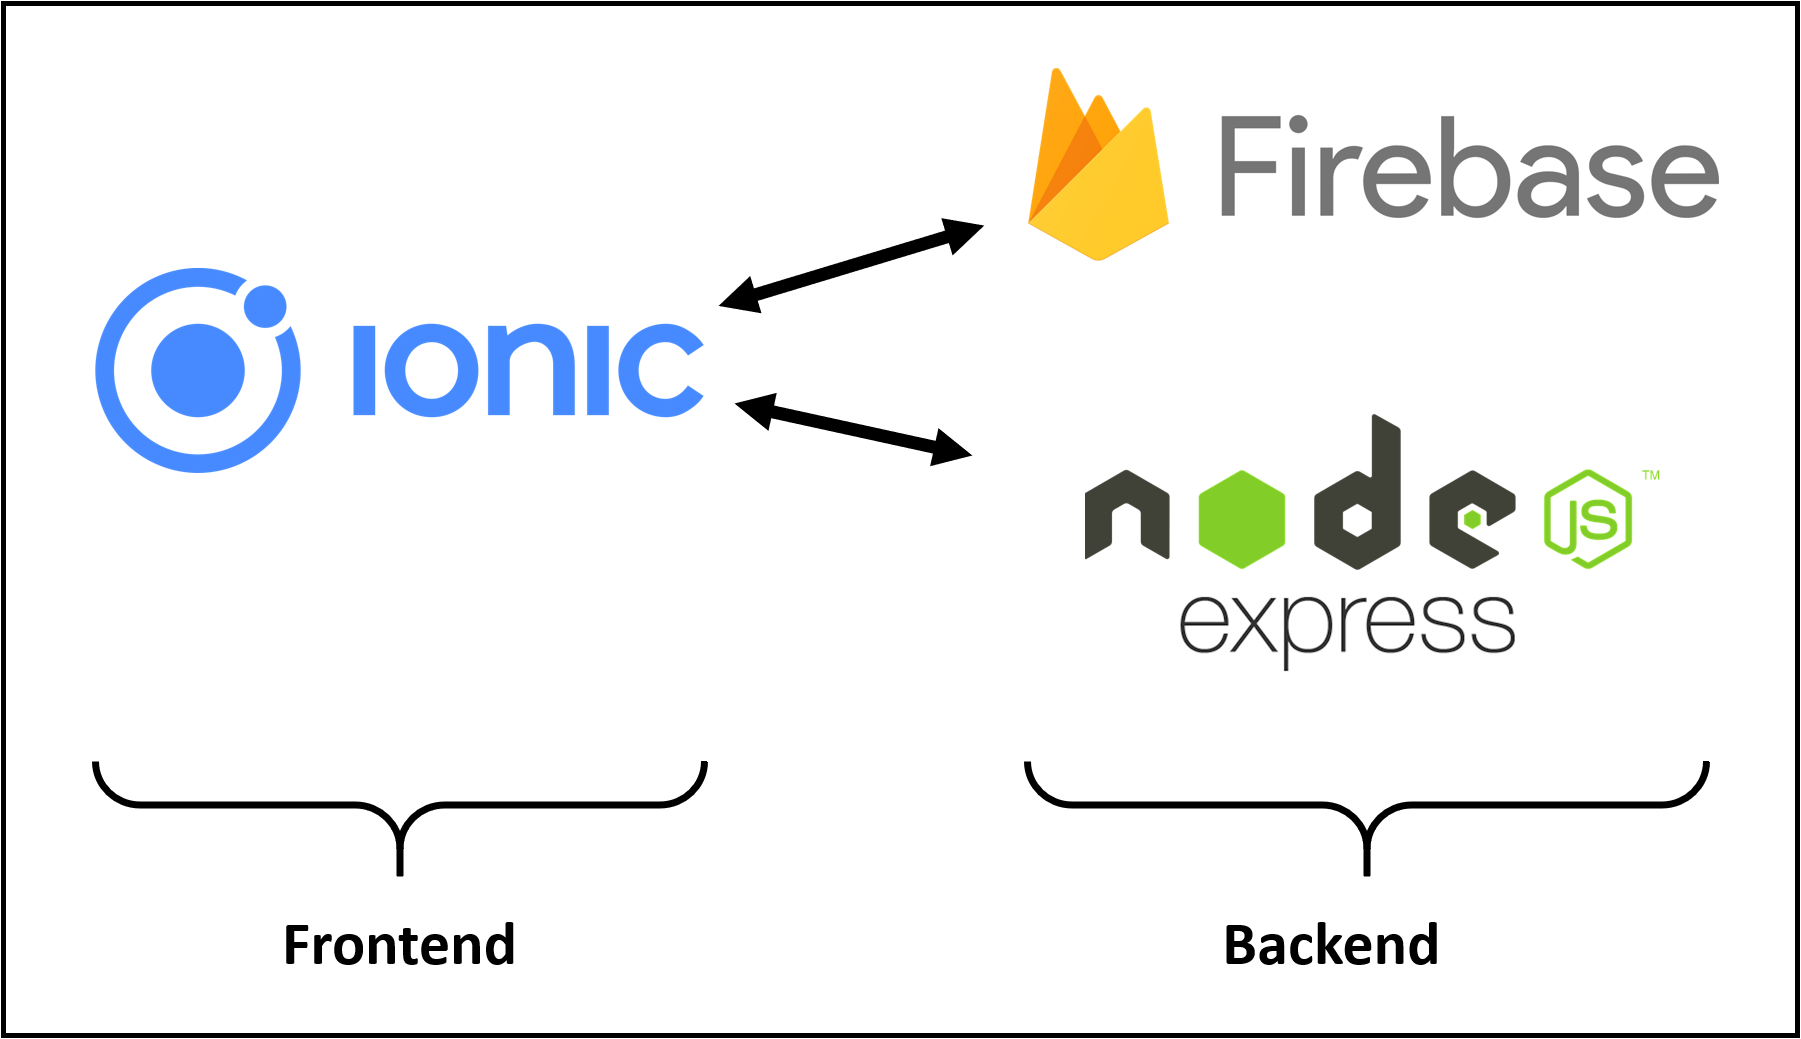
\includegraphics[width=.8\linewidth]{images/Architektur.png}
    \caption{Technologieübersicht}
    \label{fig:technologie}
\end{figure}

\section{Frontend\label{sec3.1:Unterpunkt-1}}

Inhalt

\section{Backend\label{sec3.2:Unterpunkt-2}}

Den Großteil der Backend-Aufgaben übernimmt die Entwicklungs-Platform Firebase. 